\documentclass[11pt,a4paper]{article}
\usepackage[utf8]{inputenc}
\usepackage[T1]{fontenc}
\usepackage[english]{babel}
\usepackage[a4paper,margin=2cm]{geometry}
\usepackage{titlesec}
\usepackage{tocloft}
\usepackage{amsmath,amssymb}
\usepackage{siunitx}
\usepackage{booktabs}
\usepackage{graphicx}
\usepackage{caption}
\usepackage{float}
\usepackage{subcaption}
\usepackage{enumitem}
\usepackage{xcolor}
\usepackage{tikz}
\usepackage[hidelinks]{hyperref}

\sisetup{per-mode=symbol}
\captionsetup{font=small, labelfont=bf}
\setlength{\parindent}{0pt}
\setlength{\parskip}{0.4em}
\titlespacing*{\section}{0pt}{1.6ex plus 0.3ex minus 0.2ex}{0.5ex plus 0.1ex}
\titlespacing*{\subsection}{0pt}{1.2ex plus 0.2ex minus 0.1ex}{0.3ex plus 0.1ex}
\setlength{\floatsep}{8pt plus 2pt minus 2pt}
\setlength{\textfloatsep}{8pt plus 2pt minus 2pt}
\setlength{\intextsep}{6pt plus 2pt minus 2pt}
\captionsetup{skip=3pt}
\renewcommand{\topfraction}{0.9}
\renewcommand{\bottomfraction}{0.8}
\renewcommand{\textfraction}{0.07}
\renewcommand{\floatpagefraction}{0.85}
\setcounter{tocdepth}{1}
\setlength{\cftbeforetoctitleskip}{0pt}
\setlength{\cftaftertoctitleskip}{4pt}
\setlength{\cftbeforesecskip}{1pt}
\numberwithin{equation}{section}
\graphicspath{{figures/}}

\newcommand{\er}{\mathbf{e}_r}
\newcommand{\ephi}{\mathbf{e}_\varphi}
\newcommand{\ii}{\mathbf{i}}
\newcommand{\jj}{\mathbf{j}}
\newcommand{\kk}{\mathbf{k}}
\newcommand{\rr}{\mathbf{r}}
\newcommand{\vv}{\mathbf{v}}
\newcommand{\aaa}{\mathbf{a}}
\newcommand{\NN}{\mathbf{N}}
\newcommand{\FF}{\mathbf{F}}
\newcommand{\Om}{\boldsymbol{\Omega}}
\newcommand{\dOm}{\dot{\boldsymbol{\Omega}}}
\newcommand{\dph}{\dot\varphi}
\newcommand{\ddph}{\ddot\varphi}

\begin{document}
\begin{titlepage}
\centering
\vspace*{3cm}
{\Huge\scshape Universidad Carlos III de Madrid\par}\vspace{0.4cm}
{\large Bachelor in Aerospace Engineering\par}\vspace{1.2cm}
{\Large Mechanics Applied to Aerospace Engineering\par}\vspace{0.8cm}
\rule{\linewidth}{1.2pt}\\[0.3cm]
{\LARGE\bfseries Particle on Oscillating Loop\par}\vspace{0.3cm}
\rule{\linewidth}{1.2pt}\\[0.8cm]
{\large Laboratory Session 2\par}\vspace{1.2cm}
\begin{flushleft}
\hspace{1.2cm}\textit{Authors (Laboratory Group LB):}\\
\hspace{1.2cm}Ismael Mart\'in D\'iez\\
\hspace{1.2cm}David Mart\'in Garc\'ia\\
\hspace{1.2cm}Alejandro Ranz Remart\'inez
\end{flushleft}
\vspace{1cm}{\large\textbf{Report date:} \today\par}\vfill
\end{titlepage}

\setlength{\abovedisplayskip}{5pt plus 1pt minus 1pt}
\setlength{\belowdisplayskip}{5pt plus 1pt minus 1pt}
\setlength{\abovedisplayshortskip}{2pt plus 1pt minus 1pt}
\setlength{\belowdisplayshortskip}{3pt plus 1pt minus 1pt}
\tableofcontents

\section{Introduction}
This report studies the motion of a heavy point particle $P$ of mass $m$ that slides without friction along a circular wire of centre $C$ and radius $R$ \cite{guidelines}. The wire lies in a vertical plane $Oxy$ that rotates about the vertical axis $Oy$ with the prescribed angular velocity $\Om(t)=A\omega\sin(\omega t)\,\jj$, and the position of $P$ on the wire is given by the angle $\varphi$ between $\overrightarrow{CP}$ and $Ox$ (Fig.~\ref{fig:sketch}a). The system is the one of Problem 34 of the course \cite{problems}, here solved numerically.

The difficulty is that the frame in which the motion is simple, the one attached to the wire, is not inertial and does not rotate uniformly, so the centrifugal, Euler and Coriolis forces all act on the particle. The objectives are to obtain the equation of motion and the reaction of the wire, to integrate it with \texttt{ode45} and explain the forces and the energy that result, to find an analytical criterion that separates oscillation from rotation on a fixed loop and validate it with simulations, and to determine how far a linearized equation can be trusted around the lowest point of the wire, where a resonance appears.

Section~\ref{sec:model} develops the analytical model and Section~\ref{sec:num} explains how it is implemented in Matlab. Section~\ref{sec:results} presents the results and discusses each of them next to its figure, and Section~\ref{sec:conc} gathers the conclusions.

\section{Analytical Model}\label{sec:model}
\subsection{Reference Frames and Degrees of Freedom}
The notation is that of the guidelines \cite{guidelines}. $Oxyz$ rotates with the plane of the wire: $\ii$ is horizontal along the diameter through $C$, $\jj$ is vertical and upward (the rotation axis) and $\kk=\ii\times\jj$ is normal to the plane, pointing out of the paper in Fig.~\ref{fig:sketch}a. $Ox_1y_1z_1$ is a stationary frame, assumed inertial, that coincides with $Oxyz$ at $t=0$, with $\jj_1=\jj$. The axis $Oy$ is tangent to the wire at $O$, so $\overrightarrow{OC}=R\,\ii$.

A free particle has three coordinates. The wire imposes two constraints, since $P$ must stay in the plane $Oxy$ and at distance $R$ from $C$, so the system has $3-2=1$ configuration degree of freedom, $\varphi$. The first constraint is reonomic because the plane moves with a prescribed law: the position of $P$ seen from the stationary frame depends on $\varphi$ and also explicitly on $t$.

\begin{figure}[!htb]
\centering
\begin{subfigure}[b]{0.53\textwidth}\centering
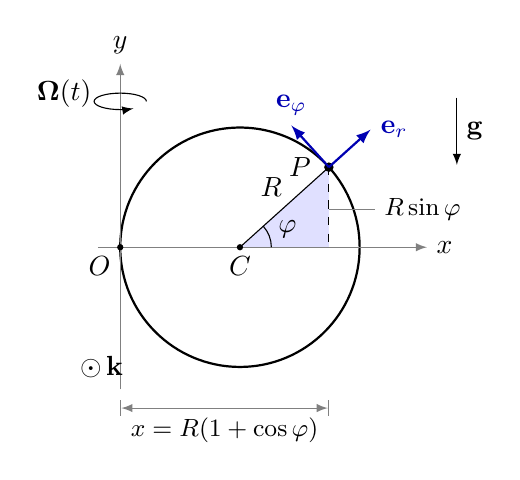
\begin{tikzpicture}[scale=0.95,>=latex]
\def\R{1.6}\def\ph{42}
\pgfmathsetmacro{\px}{\R+\R*cos(\ph)}\pgfmathsetmacro{\py}{\R*sin(\ph)}
\fill[blue!12] (\R,0) -- (\px,0) -- (\px,\py) -- cycle;
\draw[thick] (\R,0) circle (\R);
\draw[->,gray] (-0.3,0) -- (4.1,0) node[right,black] {$x$};
\draw[->,gray] (0,-1.9) -- (0,2.45) node[above,black] {$y$};
\fill (0,0) circle (1.2pt) node[below left] {$O$};
\fill (\R,0) circle (1.2pt) node[below] {$C$};
\draw (\R,0) -- (\px,\py) node[pos=0.55,above left=-1pt] {$R$};
\draw[dashed] (\px,\py) -- (\px,0);
\draw[gray,thin] (\px,0.5) -- (3.4,0.5) node[right,black] {\small $R\sin\varphi$};
\draw[|<->|,gray] (0,-2.15) -- (\px,-2.15) node[midway,below,black] {\small $x=R(1+\cos\varphi)$};
\fill (\px,\py) circle (1.8pt) node[left=3pt] {$P$};
\draw (\R+0.42,0) arc (0:\ph:0.42); \node at ({\R+0.68*cos(\ph/2)},{0.68*sin(\ph/2)}) {$\varphi$};
\draw[->,thick,blue!70!black] (\px,\py) -- ++({0.75*cos(\ph)},{0.75*sin(\ph)}) node[right] {$\er$};
\draw[->,thick,blue!70!black] (\px,\py) -- ++({-0.75*sin(\ph)},{0.75*cos(\ph)}) node[above] {$\ephi$};
\draw[->] (0.35,1.95) arc (0:300:0.35 and 0.11); \node at (-0.75,2.05) {$\Om(t)$};
\draw[->] (4.5,2.0) -- (4.5,1.1) node[midway,right] {$\mathbf{g}$};
\node at (-0.25,-1.6) {$\odot\,\kk$};
\end{tikzpicture}
\caption{Plane of the wire, $\kk$ points out of the paper.}
\end{subfigure}\hfill
\begin{subfigure}[b]{0.43\textwidth}\centering
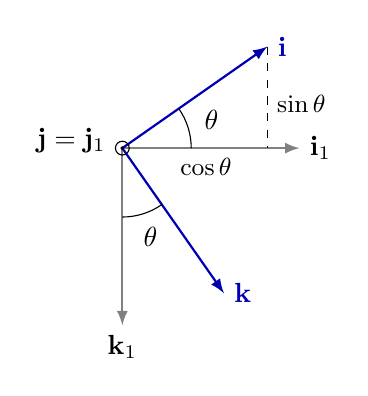
\begin{tikzpicture}[scale=1.25,>=latex]
\def\th{35}
\draw[->,thick,gray] (0,0) -- (1.8,0) node[right,black] {$\ii_1$};
\draw[->,thick,gray] (0,0) -- (0,-1.8) node[below,black] {$\kk_1$};
\draw[->,thick,blue!70!black] (0,0) -- ({1.8*cos(\th)},{1.8*sin(\th)}) node[right] {$\ii$};
\draw[->,thick,blue!70!black] (0,0) -- ({1.8*sin(\th)},{-1.8*cos(\th)}) node[right] {$\kk$};
\draw[dashed] ({1.8*cos(\th)},{1.8*sin(\th)}) -- ({1.8*cos(\th)},0);
\node[right] at ({1.8*cos(\th)},0.45) {\small $\sin\theta$};
\node[below] at (0.85,0) {\small $\cos\theta$};
\draw (0.7,0) arc (0:\th:0.7); \node at ({0.95*cos(\th/2)},{0.95*sin(\th/2)}) {$\theta$};
\draw (0,-0.7) arc (-90:{\th-90}:0.7); \node at ({0.95*sin(\th/2)},{-0.95*cos(\th/2)}) {$\theta$};
\draw (0,0) circle (0.07); \fill (0,0) circle (0.02);
\node[left] at (-0.07,0.08) {$\jj=\jj_1$};
\end{tikzpicture}
\caption{View from above, $\jj$ points out of the paper.}
\end{subfigure}
\caption{Geometry of the problem. The angle $\theta$ is the rotation of the plane about the vertical axis.}\label{fig:sketch}
\end{figure}

The angle $\theta$ turned by the plane satisfies $\dot\theta=\Omega$ with $\theta(0)=0$, where $\Omega=A\omega\sin\omega t$. Integrating with the change $u=\omega\tau$, $du=\omega\,d\tau$, and Barrow's rule:
\begin{equation}
\theta(t)=\int_0^t A\omega\sin(\omega\tau)\,d\tau=A\int_0^{\omega t}\sin u\,du=A\big[-\cos u\big]_0^{\omega t}=A\,(1-\cos\omega t),\label{eq:theta}
\end{equation}
so the plane swings between $\theta=0$ and $\theta=2A$ with period $T=2\pi/\omega$; it does not spin. For the change of basis the plane is viewed from above (Fig.~\ref{fig:sketch}b), with $\jj$ pointing towards the reader. Since $\kk_1\times\ii_1=\jj_1$, a positive rotation about $\jj_1$ takes $\kk_1$ towards $\ii_1$ and $\ii_1$ towards $-\kk_1$. The vector $\ii$ is the hypotenuse of the dashed right triangle: its leg adjacent to $\theta$ lies along $\ii_1$ and measures $\cos\theta$, and its opposite leg lies along $-\kk_1$ and measures $\sin\theta$, which is the origin of the minus sign. The same triangle applied to $\kk$ gives
\begin{equation}
\ii=\cos\theta\,\ii_1-\sin\theta\,\kk_1,\quad \jj=\jj_1,\quad \kk=\sin\theta\,\ii_1+\cos\theta\,\kk_1,\qquad
[Q]=\begin{pmatrix}\cos\theta&0&\sin\theta\\0&1&0\\-\sin\theta&0&\cos\theta\end{pmatrix},\label{eq:rot}
\end{equation}
where the columns of $[Q]$ are the components of $\ii,\jj,\kk$ in the stationary basis, $\det[Q]=\cos^2\theta+\sin^2\theta=1$ and $[Q][Q]^T=I$. As a check, the chain rule gives $d\ii/dt=-\dot\theta\,(\sin\theta\,\ii_1+\cos\theta\,\kk_1)=-\Omega\,\kk$, which is $\Om\times\ii$.

\subsection{Position, Velocity and Acceleration of $P$}
In the shaded right triangle at $C$ (Fig.~\ref{fig:sketch}a) the hypotenuse is $R$, the leg adjacent to $\varphi$ is $R\cos\varphi$ along $\ii$ and the opposite one is $R\sin\varphi$ along $\jj$. Then, with $x\equiv R(1+\cos\varphi)$ the distance from $P$ to the rotation axis,
\begin{equation}
\rr=\overrightarrow{OC}+\overrightarrow{CP}=R(1+\cos\varphi)\,\ii+R\sin\varphi\,\jj=x\,\ii+R\sin\varphi\,\jj .\label{eq:r}
\end{equation}
The polar basis is $\er=\cos\varphi\,\ii+\sin\varphi\,\jj$, $\ephi=-\sin\varphi\,\ii+\cos\varphi\,\jj$. In $Oxyz$ the vectors $\ii,\jj$ are constant and only $\varphi$ depends on time. The chain rule, $\frac{d}{dt}\cos\varphi=-\dph\sin\varphi$ and $\frac{d}{dt}\sin\varphi=\dph\cos\varphi$, gives the relative velocity, and the product rule, $\frac{d}{dt}(\dph\sin\varphi)=\ddph\sin\varphi+\dph^2\cos\varphi$ and $\frac{d}{dt}(\dph\cos\varphi)=\ddph\cos\varphi-\dph^2\sin\varphi$, the relative acceleration:
\begin{align}
\vv_{rel}&=-R\dph\sin\varphi\,\ii+R\dph\cos\varphi\,\jj=R\dph\,\ephi,\label{eq:vrel}\\
\aaa_{rel}&=-R(\ddph\sin\varphi+\dph^2\cos\varphi)\,\ii+R(\ddph\cos\varphi-\dph^2\sin\varphi)\,\jj=R\ddph\,\ephi-R\dph^2\,\er .\label{eq:arel}
\end{align}
For the motion of the frame, $O$ is fixed, $\Om=\Omega\,\jj$ and $\dOm=\dot\Omega\,\jj$ with $\dot\Omega=A\omega^2\cos\omega t$, because $\jj$ does not change. With $\jj\times\ii=-\kk$, $\jj\times\jj=\mathbf{0}$ and $\jj\times\kk=\ii$:
\begin{equation}
\begin{aligned}
\Om\times\rr&=\Omega\,\jj\times(x\,\ii+R\sin\varphi\,\jj)=-\Omega x\,\kk,\qquad \dOm\times\rr=-\dot\Omega x\,\kk,\\
\Om\times(\Om\times\rr)&=\Omega\,\jj\times(-\Omega x\,\kk)=-\Omega^2x\,\ii,\\
2\Om\times\vv_{rel}&=2\Omega R\dph\,\jj\times(-\sin\varphi\,\ii+\cos\varphi\,\jj)=2\Omega R\dph\sin\varphi\,\kk .
\end{aligned}\label{eq:cross}
\end{equation}
The composition of motions \cite[Eqs.~3.26--3.27]{notes} gives the velocity and acceleration in the stationary frame:
\begin{align}
\vv&=\vv_{rel}+\Om\times\rr=R\dph\,\ephi-\Omega x\,\kk,\label{eq:vabs}\\
\aaa&=\big[-R(\ddph\sin\varphi+\dph^2\cos\varphi)-\Omega^2x\big]\ii+R(\ddph\cos\varphi-\dph^2\sin\varphi)\,\jj+\big[2\Omega R\dph\sin\varphi-\dot\Omega x\big]\kk .\label{eq:aabs}
\end{align}

\subsection{Forces on the Particle}
Two real forces act on $P$: its weight and the reaction of the wire. The wire is smooth, so the reaction has no component along the tangent $\ephi$:
\begin{equation}
m\mathbf{g}=-mg\,\jj=-mg\,(\sin\varphi\,\er+\cos\varphi\,\ephi),\qquad \NN=N_1\,\er+N_2\,\kk .\label{eq:real}
\end{equation}
Since $Oxyz$ is not inertial, the inertia forces must be added \cite[Eqs.~4.62--4.63]{notes}. From Eq.~\eqref{eq:cross} and $\ii=\cos\varphi\,\er-\sin\varphi\,\ephi$:
\begin{align}
\FF_{cent}&=-m\Om\times(\Om\times\rr)=m\Omega^2x\,\ii=mA^2\omega^2R\sin^2(\omega t)(1+\cos\varphi)\,[\cos\varphi\,\er-\sin\varphi\,\ephi],\label{eq:Fcent}\\
\FF_{Euler}&=-m\dOm\times\rr=m\dot\Omega x\,\kk=mA\omega^2R\cos(\omega t)(1+\cos\varphi)\,\kk,\label{eq:Feul}\\
\FF_{Cor}&=-2m\Om\times\vv_{rel}=-2mA\omega R\dph\sin(\omega t)\sin\varphi\,\kk .\label{eq:Fcor}
\end{align}

\subsection{Equation of Motion and Reaction Forces}
In $Oxyz$, $m\aaa_{rel}=m\mathbf{g}+\NN+\FF_{cent}+\FF_{Euler}+\FF_{Cor}$. The direction $\ephi$ contains no reaction, and the Euler and Coriolis forces are along $\kk$, so projecting on $\ephi$ gives $mR\ddph=-mg\cos\varphi-m\Omega^2x\sin\varphi$, that is
\begin{equation}
\boxed{\ddph=-\frac{g}{R}\cos\varphi-A^2\omega^2\sin^2(\omega t)\,(1+\cos\varphi)\sin\varphi}\label{eq:eom}
\end{equation}
The other two projections give the reactions. On $\er$, $-mR\dph^2=N_1-mg\sin\varphi+m\Omega^2x\cos\varphi$, and on $\kk$, $0=N_2+m\dot\Omega x-2m\Omega R\dph\sin\varphi$:
\begin{align}
N_1&=-mR\dph^2+mg\sin\varphi-mA^2\omega^2R\sin^2(\omega t)(1+\cos\varphi)\cos\varphi,\label{eq:N1}\\
N_2&=mA\omega R\big[2\dph\sin(\omega t)\sin\varphi-\omega\cos(\omega t)(1+\cos\varphi)\big].\label{eq:N2}
\end{align}
All the terms are homogeneous: $[g/R]=[\Omega^2]=\si{s^{-2}}=[\ddph]$ in Eq.~\eqref{eq:eom}, and $[mR\dph^2]=[mg]=[mA\omega^2R]=\si{N}$ in the reactions. Equations~\eqref{eq:eom}--\eqref{eq:N2} agree with the official key of Problem 34 \cite{problems} and with the slides \cite{slides}. For $A=0$, Eq.~\eqref{eq:eom} is a pendulum with its stable equilibrium at the bottom, $\varphi=-\pi/2$, and the unstable one at the top, $\varphi=\pi/2$.

\subsection{Mechanical Energy and Work of the Wire}
With Eq.~\eqref{eq:vabs}, where $\ephi\perp\kk$, and taking the height of $O$ as the reference,
\begin{equation}
E_k=\tfrac12 m\big(R^2\dph^2+\Omega^2x^2\big),\qquad E_p=mgR\sin\varphi,\qquad E=E_k+E_p .\label{eq:E}
\end{equation}
By the work--energy theorem $dE_k/dt=(m\mathbf{g}+\NN)\cdot\vv$, and the weight is conservative, $m\mathbf{g}\cdot\vv=-dE_p/dt$. Only the power of the reaction is left, and since $\er\perp\ephi$ and $\er\perp\kk$,
\begin{equation}
\frac{dE}{dt}=\NN\cdot\vv=(N_1\er+N_2\kk)\cdot(R\dph\,\ephi-\Omega x\,\kk)=-\Omega x N_2 .\label{eq:Edot}
\end{equation}
On a fixed wire the reaction is perpendicular to the velocity. Here the wire moves with the plane, so $N_2$ does work and $E$ is conserved if and only if $A=0$. From Eq.~\eqref{eq:N2}, using $\dot x=-R\dph\sin\varphi$, the torque of the wire about the axis is
\begin{equation}
-xN_2=2m\Omega x\dot x+m\dot\Omega x^2=\frac{d}{dt}\big(m\Omega x^2\big),\label{eq:torque}
\end{equation}
the rate of change of the angular momentum of $P$ about the axis, $L=m\Omega x^2$, so that $dE/dt=\Omega\,dL/dt$. In $Oxyz$ the energy includes the centrifugal potential instead, and it changes only because $\Omega$ varies:
\begin{equation}
J=E-\Omega L=\tfrac12mR^2\dph^2+E_p-\tfrac12m\Omega^2x^2,\qquad \frac{dJ}{dt}=-\dot\Omega L,\qquad E=J+m\Omega^2x^2 .\label{eq:J}
\end{equation}

\subsection{Fixed Loop: Criterion for the Motion}\label{sec:crit}
For $A=0$, multiplying Eq.~\eqref{eq:eom} by $\dph$ gives $\dph\ddph+(g/R)\cos\varphi\,\dph=0$. By the chain rule this is a total derivative, $\frac{d}{dt}\big[\tfrac12\dph^2+\tfrac{g}{R}\sin\varphi\big]=0$, and applying Barrow's rule between $0$ and $t$:
\begin{equation}
\tfrac12\dph^2+\frac gR\sin\varphi=\tfrac12\dph_0^2+\frac gR\sin\varphi_0=\frac{E_0}{mR^2} .\label{eq:first}
\end{equation}
The potential energy has its maximum, $mgR$, at the top of the loop, $\varphi=\pi/2$. If $E_0>mgR$, $P$ reaches the top with $\dph\neq0$, $\dph$ never changes sign and $\varphi$ grows (or decreases) steadily. If $E_0<mgR$, $\dph$ vanishes before the top and $\varphi$ oscillates. Imposing $E_0>mgR$ in Eq.~\eqref{eq:first}, $\varphi$ rotates if
\begin{equation}
|\dph_0|>\dph_c(\varphi_0)=\sqrt{\frac{2g}{R}\big(1-\sin\varphi_0\big)} ,\label{eq:crit}
\end{equation}
with $\dph_0>0$ for a growing $\varphi$. Otherwise $\dph=0$ in Eq.~\eqref{eq:first} gives the turning points, $\varphi_{max}=\arcsin\big(\sin\varphi_0+R\dph_0^2/(2g)\big)$ and $\varphi_{min}=-\pi-\varphi_{max}$. The limit $E_0=mgR$ is the separatrix $\dph=\pm\sqrt{(2g/R)(1-\sin\varphi)}$, along which the top is only approached in an infinite time: near it $\epsilon=\pi/2-\varphi$ follows $\dot\epsilon\approx-\sqrt{g/R}\,\epsilon$.

\subsection{Linearized Equation}\label{sec:lin}
With $\varphi=\delta-\pi/2$, $\cos\varphi=\sin\delta$, $\sin\varphi=-\cos\delta$ and $\ddph=\ddot\delta$, so Eq.~\eqref{eq:eom} becomes the exact $\ddot\delta=-(g/R)\sin\delta+\Omega^2(1+\sin\delta)\cos\delta$. For $\delta\ll1$, $\sin\delta\approx\delta$ and $\cos\delta\approx1$, which gives $\ddot\delta=-(g/R)\delta+\Omega^2(1+\delta)$. The hypothesis $A^2\ll g/(R\omega^2)$ means $\Omega^2\le A^2\omega^2\ll g/R$, so $\Omega^2\delta$ is dropped against $(g/R)\delta$ \cite{slides}. Using $\sin^2\omega t=\tfrac12(1-\cos2\omega t)$:
\begin{equation}
\ddot\delta+\frac gR\,\delta-\Omega^2=0\quad\Longleftrightarrow\quad\ddot\delta+\omega_n^2\delta=F_0\,(1-\cos2\omega t),\qquad \omega_n=\sqrt{g/R},\quad F_0=\tfrac12A^2\omega^2 .\label{eq:lin}
\end{equation}
This is an undamped oscillator forced at the frequency $2\omega$ by the centrifugal force, which peaks twice per period of the plane. The guidelines give no initial conditions, so $P$ is taken at rest at the bottom, $\delta(0)=\dot\delta(0)=0$, and all the motion comes from the loop. The constant $F_0/\omega_n^2$ and $C\cos2\omega t$ with $C=-F_0/(\omega_n^2-4\omega^2)$ are a particular solution; adding $a\cos\omega_nt+b\sin\omega_nt$ and imposing the initial conditions:
\begin{equation}
\delta=\frac{F_0}{\omega_n^2}-\frac{F_0\cos2\omega t}{\omega_n^2-4\omega^2}+\Big(\frac{F_0}{\omega_n^2-4\omega^2}-\frac{F_0}{\omega_n^2}\Big)\cos\omega_nt,\qquad 2\omega\neq\omega_n .\label{eq:linsol}
\end{equation}
Thus $P$ oscillates around $\delta_s=F_0/\omega_n^2=A^2R\omega^2/(2g)$, displaced outwards from the bottom. If $2\omega=\omega_n$ the denominator vanishes. This is resonance \cite[Sec.~5.4.1]{notes}, and the particular solution changes to $-\frac{F_0}{2\omega_n}t\sin\omega_nt$, which satisfies $\ddot\delta+\omega_n^2\delta=-F_0\cos\omega_nt$:
\begin{equation}
\delta=\frac{F_0}{\omega_n^2}(1-\cos\omega_nt)-\frac{F_0}{2\omega_n}\,t\sin\omega_nt,\qquad 2\omega=\omega_n .\label{eq:res}
\end{equation}
The amplitude grows linearly with time, so $\delta\ll1$ stops holding at $\omega=\tfrac12\sqrt{g/R}$.

\section{Numerical Implementation in Matlab}\label{sec:num}
Equation~\eqref{eq:eom} is written for the state vector $X=[\varphi,\dph]^T=[X_1,X_2]^T$ because \texttt{ode45} \cite{matlab} integrates first-order systems:
\begin{equation}
\frac{d}{dt}\begin{pmatrix}X_1\\X_2\end{pmatrix}=f(t,X)=\begin{pmatrix}X_2\\[2pt]-\dfrac gR\cos X_1-A^2\omega^2\sin^2(\omega t)\,(1+\cos X_1)\sin X_1\end{pmatrix} .\label{eq:state}
\end{equation}
This is the function \texttt{diffeq(t,X,g,omega,R,A)} of \texttt{main.m}, and Eq.~\eqref{eq:lin} is \texttt{diffeqlin}, with $X=[\delta,\dot\delta]^T$. The options are \texttt{RelTol} $=10^{-8}$, \texttt{AbsTol} $=10^{-10}$ (the default $10^{-6}$ is not small against $\delta\sim10^{-3}$) and \texttt{MaxStep} $=\SI{0.01}{s}$, at least 237 steps per swing, far above the Nyquist limit \cite{guidelines}. The forces and energies are computed afterwards from $\varphi$ and $\dph$ with Eqs.~\eqref{eq:Fcent}--\eqref{eq:N2} and \eqref{eq:E}, and the work of the wire $W_N$ with the trapezoidal rule applied to Eq.~\eqref{eq:Edot}. The position in the stationary frame follows from Eqs.~\eqref{eq:theta}--\eqref{eq:r}: $x_1=x\cos\theta$, $y_1=R\sin\varphi$, $z_1=-x\sin\theta$. A fixed-loop case counts as rotating if $\dph$ never changes sign and as oscillating otherwise, and the periods come from the times of the extrema of $\varphi$. Every number quoted in this report is printed by \texttt{main.m}.

In all cases $g=\SI{9.81}{m/s^2}$ and $m=\SI{1}{kg}$. The oscillating loop uses $A=\pi$, $R=\SI{1}{m}$, $\omega=\SI{0.1}{rad/s}$, $\varphi(0)=\dph(0)=0$ and $t\in[0,3T]$ with $T=\SI{62.83}{s}$. The fixed loop uses $A=0$ and $R=\SI{1}{m}$, and the linearized study $A=0.1$, $R=\SI{0.01}{m}$ and $\omega_n=\SI{31.32}{rad/s}$. The guidelines do not fix the duration of these two studies, so we take $t\in[0,10]$~s, longer than any period of the fixed loop and about 50 natural periods of the linearized study.

\section{Results and Discussion}\label{sec:results}
\subsection{Angle and Reaction Forces}
Figure~\ref{fig:angle} shows $\varphi$, $N_1$ and $N_2$ over $[0,3T]$ and, since the 79.5 swings of that interval cannot be followed one by one, a window of \SI{10}{s} around $t=T/4$, when the plane turns fastest. At $t=0$ the plane is at rest and Eq.~\eqref{eq:eom} gives $\ddph(0)=-g/R=\SI{-9.81}{rad/s^2}$: $P$ falls from the end of the horizontal diameter and swings around the bottom between $\varphi\approx0$ and $\varphi\approx-\pi$, the point $O$. The amplitude does not change over the three periods although $A=\pi$ is a large rotation, because what enters Eq.~\eqref{eq:eom} is $A\omega$: $\Omega^2$ is at most $(A\omega)^2$, 1.01\% of $g/R$. So $P$ behaves as a pendulum of \ang{90} amplitude. Its swing period, \SI{2.370}{s}, is longer than the small-oscillation value $2\pi\sqrt{R/g}=\SI{2.006}{s}$ and close to the exact \SI{2.368}{s} of that pendulum. The highest angle, \SI{0.0118}{rad}, puts $P$ \SI{0.0118}{m} above its start, using energy given by the wire (Section~\ref{sec:energy}).

\begin{figure}[!htb]
\centering
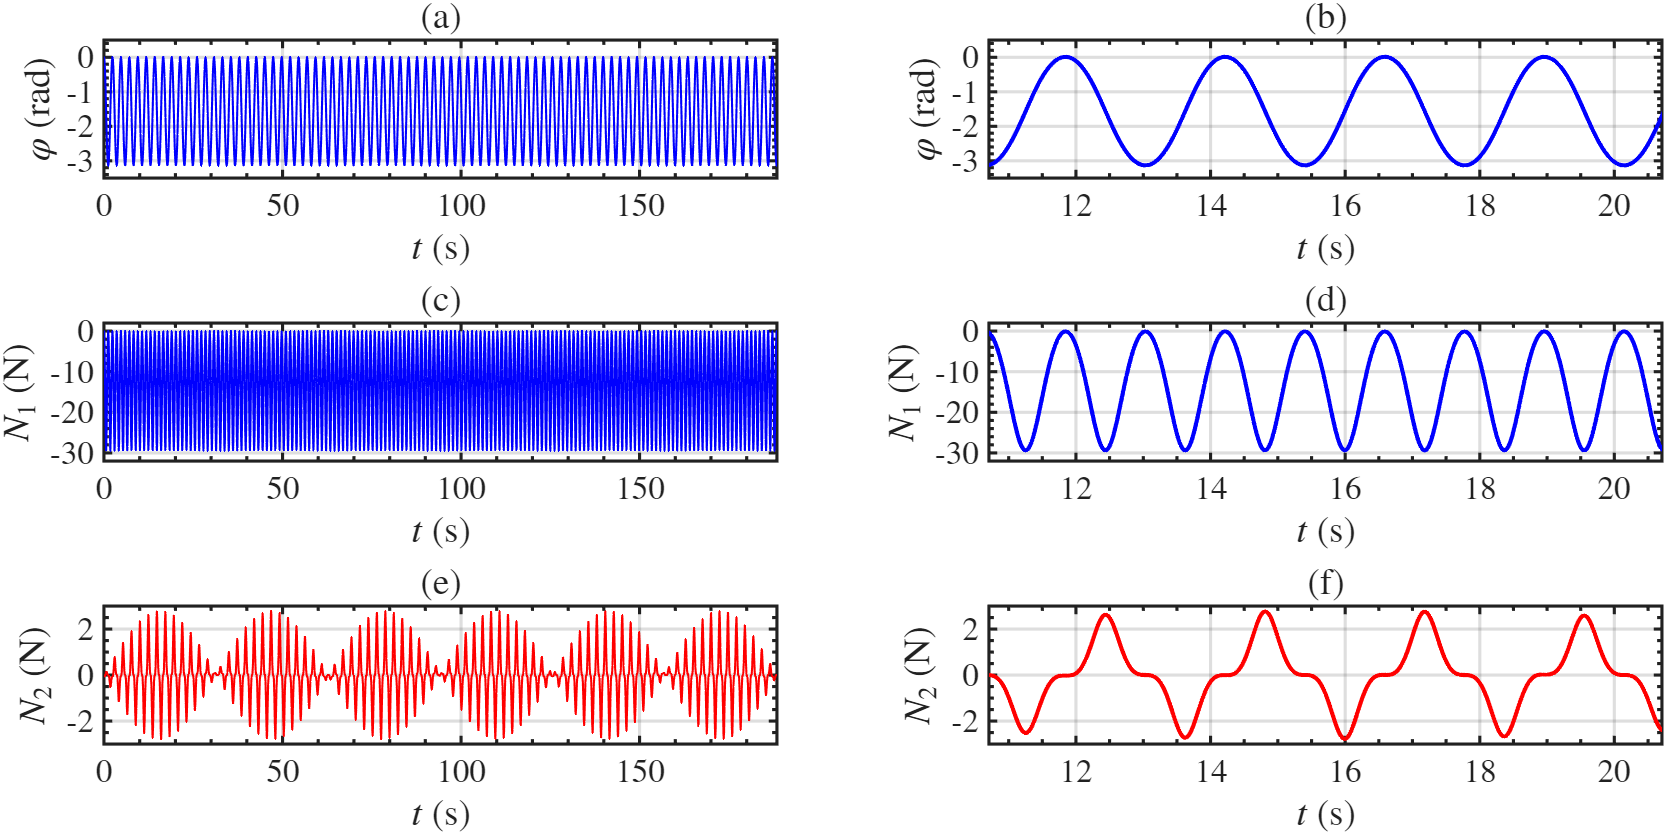
\includegraphics[width=\textwidth]{angle_reactions.png}
\caption{Oscillating loop. Left: $t\in[0,3T]$. Right: window around $t=T/4$. (a, b) Angle; (c, d) reaction along $\er$; (e, f) reaction along $\kk$.}\label{fig:angle}
\end{figure}

$N_1$ stays between \SI{-29.43}{N} and \SI{0.00}{N}, so the wire pulls $P$ towards $C$. It vanishes at the turning points, where $\dph=0$ and $\sin\varphi\approx0$, and its minimum is at the bottom: since the rotation is weak, Eq.~\eqref{eq:first} holds approximately and gives $\dph^2\approx2g/R$, and Eq.~\eqref{eq:N1} gives $N_1\approx-2mg-mg=-3mg$, the weight plus the force that makes $P$ turn. As this happens at every crossing of the bottom, $N_1$ oscillates twice as fast as $\varphi$ (Fig.~\ref{fig:angle}d). $N_2$ is 10.6 times smaller, between \SI{-2.777}{N} and \SI{2.778}{N}. Its envelope has period $T/2$ and falls to the Euler force alone when the plane stops and turns back. Inside a swing it peaks at the bottom, where $\dph$ is largest, and its sign alternates between consecutive crossings because $P$ crosses in opposite directions (Fig.~\ref{fig:angle}f). The next section shows why.

\subsection{Inertia Forces}
The three forces have different sizes, so each has its own axis in Fig.~\ref{fig:inertia}, as the guidelines require. $F_{cent}$ always points away from the axis. Its peak, \SI{0.1974}{N}, is $2mA^2\omega^2R$, reached with $P$ at $x=2R$ when $|\Omega|$ is maximum, and it is only 2.01\% of the weight. $F_{Euler}$ follows $\cos\omega t$ and is largest (\SI{0.0628}{N}) when the plane stops and $F_{cent}$ and $F_{Cor}$ vanish, since it depends on the change of $\Omega$ and not on its value. $F_{Cor}$ is the largest, up to \SI{2.778}{N}, 44.2 times $F_{Euler}$, because $P$ moves fast along the wire ($|\dph|\le\SI{4.430}{rad/s}$) compared with the slow plane ($\omega=\SI{0.1}{rad/s}$).

\begin{figure}[!htb]
\centering
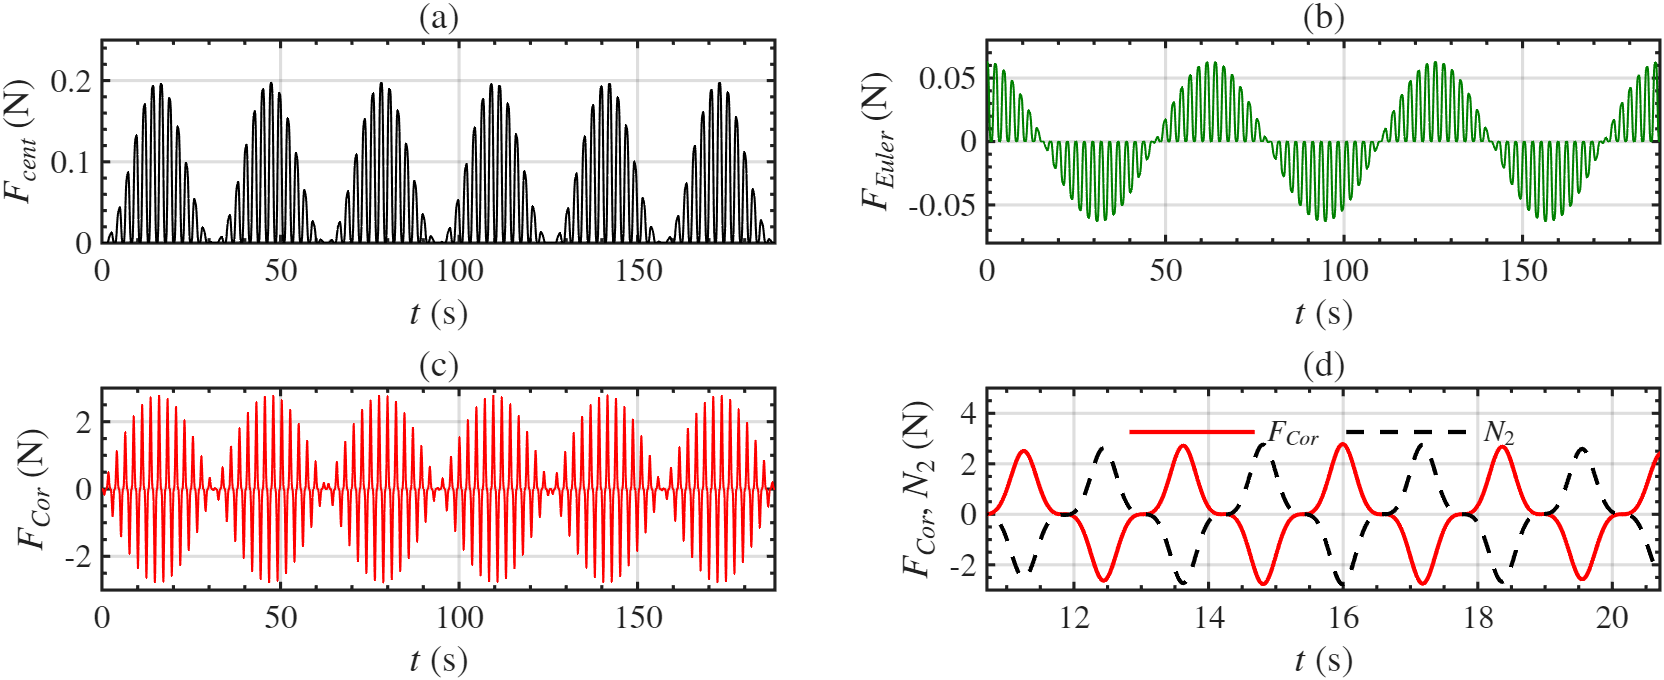
\includegraphics[width=\textwidth]{inertia_forces.png}
\caption{Inertia forces of the oscillating loop. (a) Centrifugal (along $\ii$), (b) Euler and (c) Coriolis (along $\kk$) for $t\in[0,3T]$. (d) Coriolis force and reaction $N_2$ around $t=T/4$.}\label{fig:inertia}
\end{figure}

Equation~\eqref{eq:N2} is $N_2=-F_{Cor}-F_{Euler}$, so the wire has to balance both, and since the Euler force is small $N_2$ is almost the mirror image of $F_{Cor}$ (Fig.~\ref{fig:inertia}d). So the largest inertia force does not change $\varphi$: it is normal to the plane of motion, it only loads the wire and, through $N_2$, it sets the energy exchange of Section~\ref{sec:energy}. The only inertia force in Eq.~\eqref{eq:eom} is the part of the centrifugal one along $\ephi$, which is why the swing of Fig.~\ref{fig:angle}a is almost unaffected by the rotation.

\subsection{Energy}\label{sec:energy}
In Fig.~\ref{fig:energy}(a, b) $E_k\in[0.000,9.830]$~J and $E_p\in[-9.810,0.115]$~J exchange about \SI{9.8}{J} in each half swing, as in any pendulum. Their sum is not constant: $E-E_0$ moves between \SI{-0.0824}{J} and \SI{0.3129}{J} (Fig.~\ref{fig:energy}c), as Eq.~\eqref{eq:Edot} predicts. The work $W_N$ computed from the power $-\Omega xN_2$ reproduces $E-E_0$ within \num{2.4e-6}~J, which validates $N_2$, $E$ and the integration at once.

\begin{figure}[!htb]
\centering
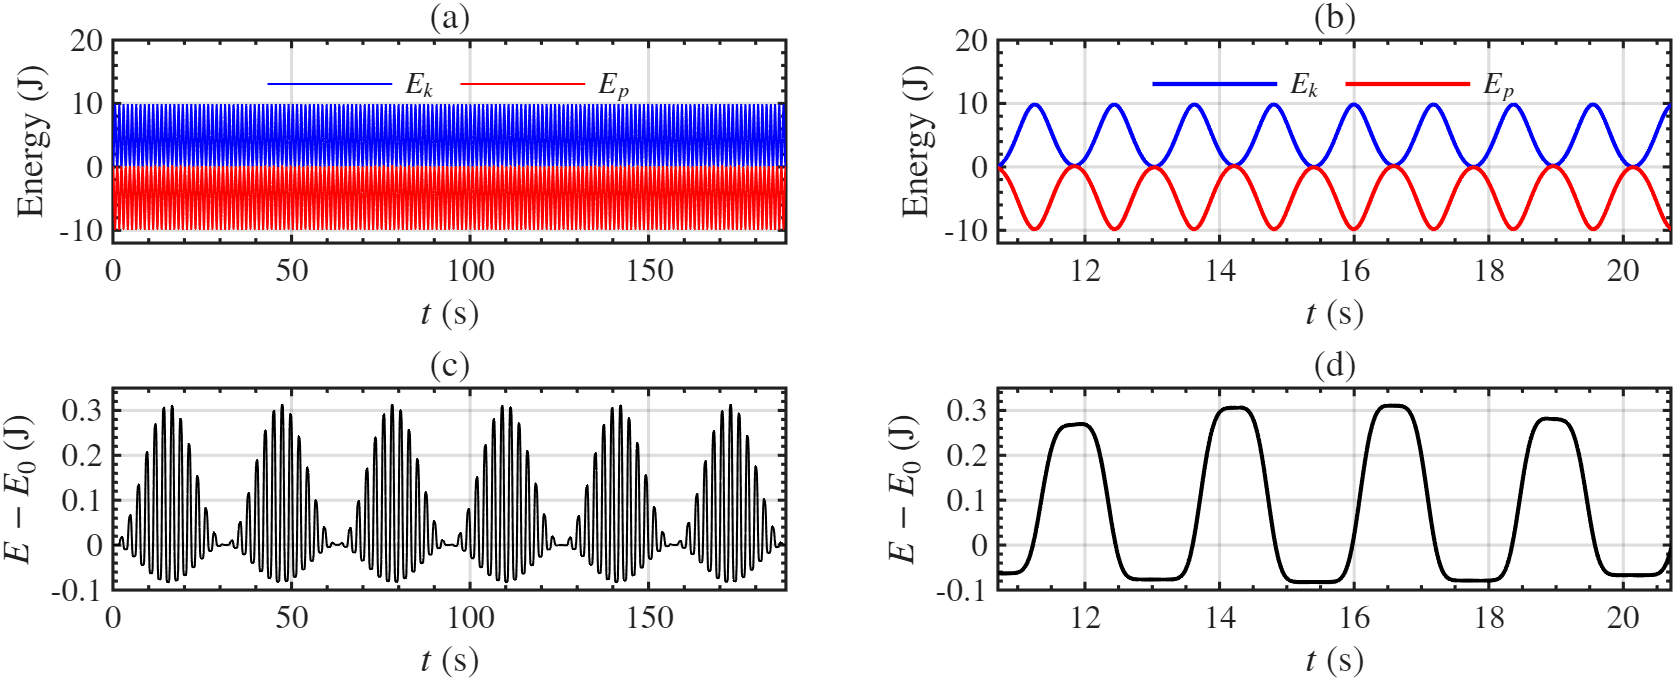
\includegraphics[width=\textwidth]{energies.png}
\caption{Energy of the oscillating loop. (a, b) Kinetic and gravitational potential energy; (c, d) change of the mechanical energy. Left: $t\in[0,3T]$. Right: window around $t=T/4$.}\label{fig:energy}
\end{figure}

Figure~\ref{fig:energy}d shows the cause: $E$ is high while $P$ is far from the axis and low while it is near. While $P$ moves outwards at an almost constant $\Omega$, the wire must increase $L=m\Omega x^2$ and the motor gives the energy $\Omega\,\Delta L$ (Eq.~\eqref{eq:torque}); it takes it back when $P$ returns. From $x=0$ to $x=2R$ at the maximum $\Omega$ this is $4mA^2\omega^2R^2=\SI{0.3948}{J}$, and the range of $E$ in the simulation is \SI{0.3953}{J}. $E$ also falls below $E_0$, which Eq.~\eqref{eq:J} explains. As $\Omega$ varies slowly compared with the swing, $J$ follows $-\tfrac12m\Omega^2\langle x^2\rangle$, with $\langle x^2\rangle=\SI{1.670}{m^2}$ the average over the swing. At the maximum $\Omega$ this predicts $E-E_0=\SI{-0.0824}{J}$ at $x=0$ and \SI{0.3124}{J} at $x=2R$, as simulated. When the plane stops, $\Omega=0$ and $J$ returns to almost zero, so there is no net gain after each of its periods (26.5 swings): $E-E_0$ is \SI{0.0006}{J} at $T$, \SI{0.0000}{J} at $2T$ and \SI{0.0006}{J} at $3T$. This is why the amplitude of Fig.~\ref{fig:angle}a does not drift.

\subsection{Trajectory in the Stationary Frame}
From the ground (Fig.~\ref{fig:traj}), $P$ moves on the surface swept by the wire, a torus without a hole because the circle touches the axis: the distance to the axis goes from practically zero (\num{1.0e-12}~m) to \SI{2.0000}{m}. Each swing draws one petal from the axis to $x=2R$ and back, and the plane spreads them around the axis because it turns up to $\theta=2A=2\pi$ at $t=T/2$ and back to $0$ at $t=T$. The petals are not evenly spaced because of the law of $\Omega$. Near $\theta=0$ and $\theta=2\pi$ the plane is almost stopped, so the petals bunch around $+x_1$ (Fig.~\ref{fig:traj}b); near $\theta=\pi$ it turns fastest, up to \SI{0.744}{rad} per swing, and they open up. The three periods give almost the same flower, slightly displaced because $T$ is not a multiple of the swing period. The video \texttt{trajectory\_video.avi} (generated by \texttt{main.m}) shows the first period with the wire moving.

\begin{figure}[!htb]
\centering
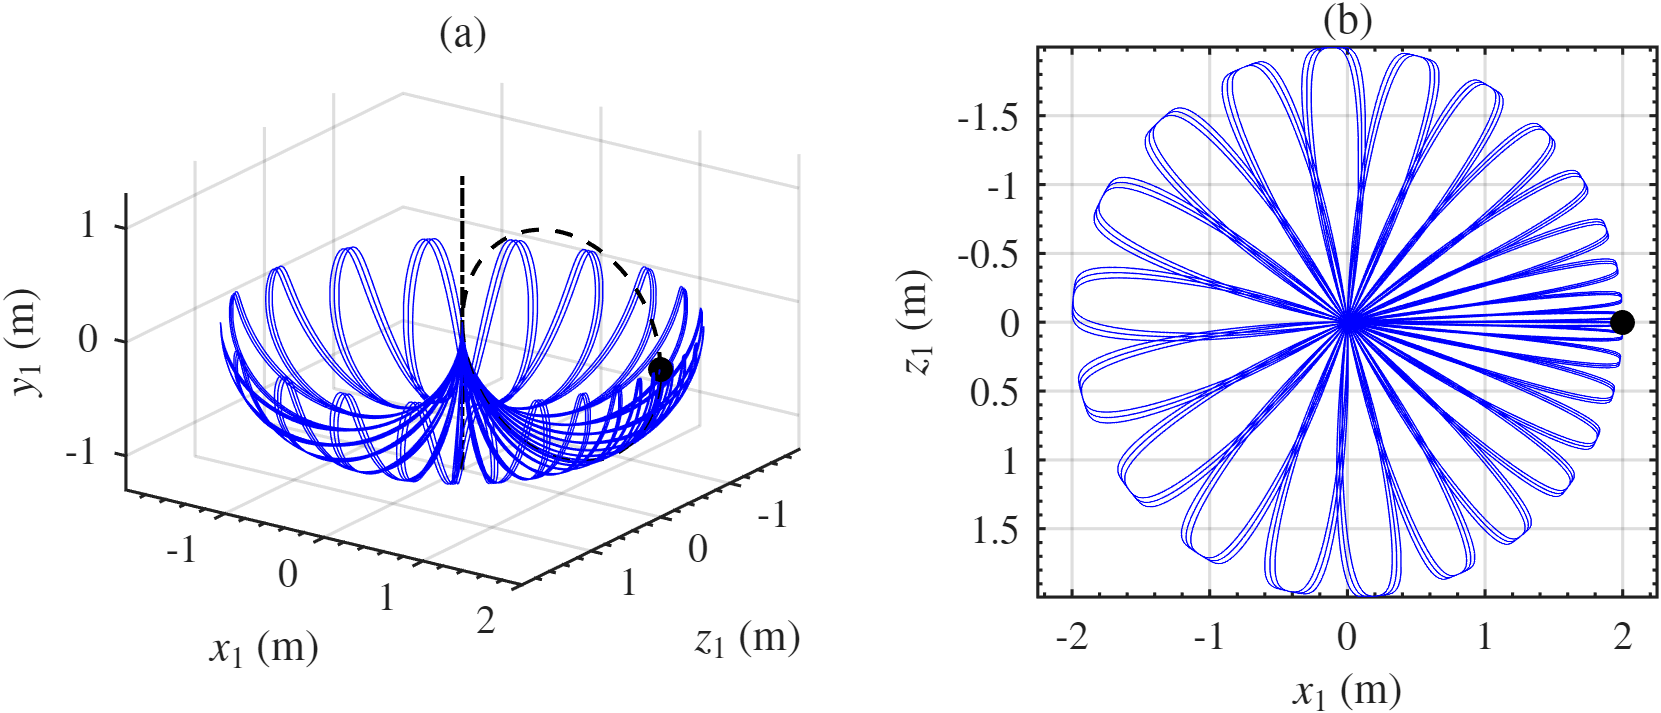
\includegraphics[width=\textwidth]{trajectory.png}
\caption{Trajectory of $P$ in $Ox_1y_1z_1$ for $t\in[0,3T]$, with the start marked by a dot. (a) Three-dimensional view with the wire at $t=0$ (dashed) and the rotation axis (dash-dot). (b) View from above, with $z_1$ pointing down as in Fig.~\ref{fig:sketch}b.}\label{fig:traj}
\end{figure}

\subsection{Fixed Loop: Phase Portrait and Validation of the Criterion}
Figure~\ref{fig:phase} shows the nine initial conditions together with the separatrix of Eq.~\eqref{eq:crit}, and Table~\ref{tab:phase} compares the analytical prediction with the simulation. $\varphi$ is plotted modulo $2\pi$, so both ends of the axis are the top of the loop. The prediction and the simulation agree in all nine cases, and $\varphi_{max}$ agrees with the formula of Section~\ref{sec:crit} to all the digits shown. As Eq.~\eqref{eq:first} requires, $E$ is conserved, here within \num{4.0e-10}~$mgR$, which also shows that the numerical error is negligible.

\begin{figure}[!htb]
\centering
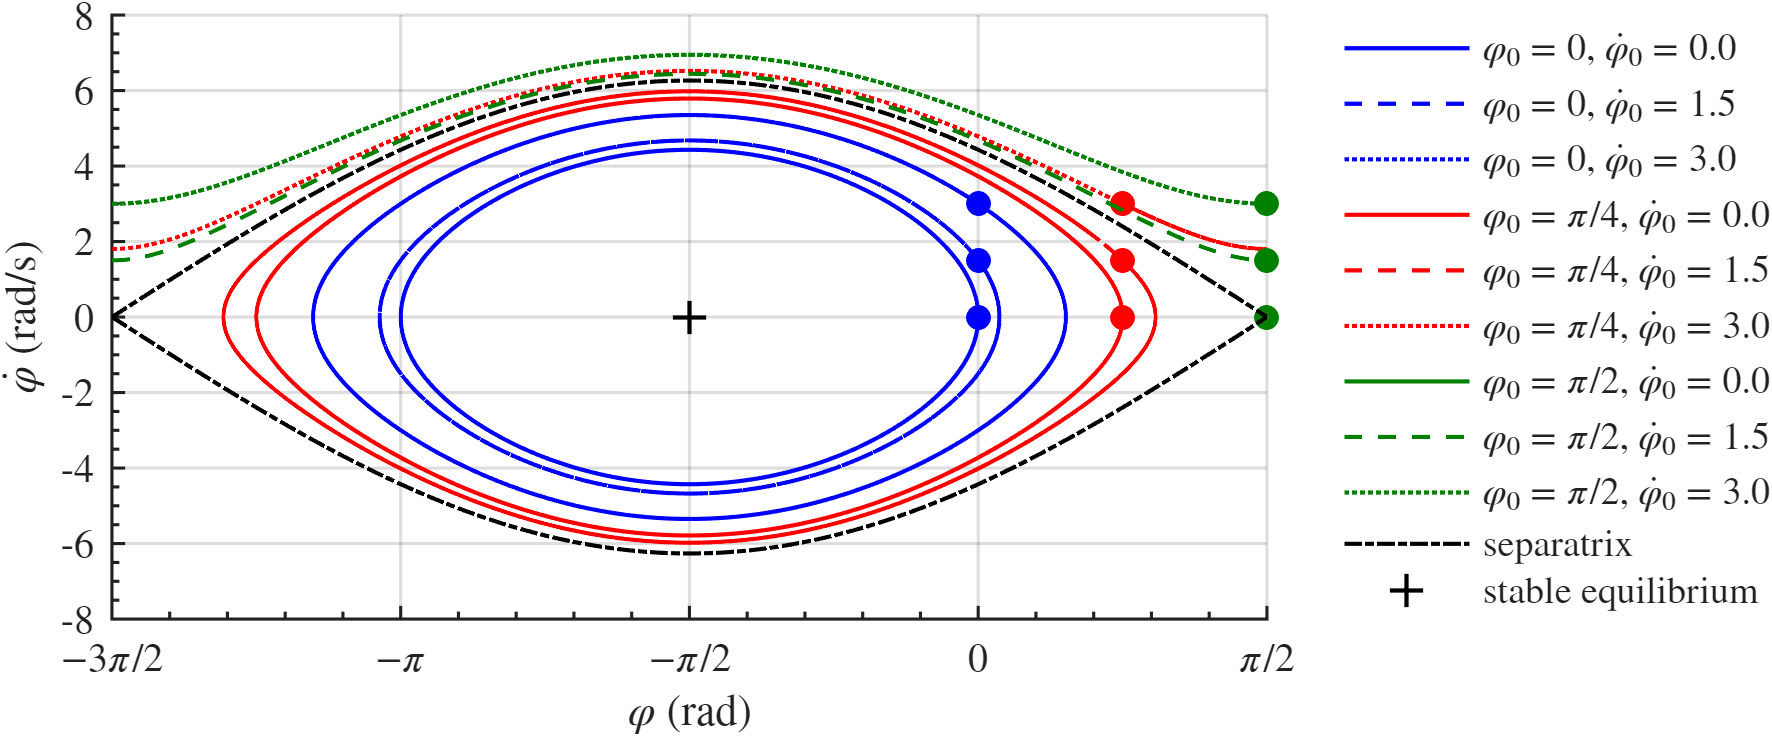
\includegraphics[width=\textwidth]{phase_portrait.png}
\caption{Phase portrait of the fixed loop ($A=0$), with $\varphi_0$ in rad and $\dph_0$ in rad/s. Dots mark the initial conditions and the dash-dot line is the separatrix. Closed curves are oscillations and open curves are rotations.}\label{fig:phase}
\end{figure}

\begin{table}[!htb]
\centering\small
\caption{Criterion of Eq.~\eqref{eq:crit} against the simulation of the fixed loop. $\varphi_{max}$ and the period come from the simulation.}\label{tab:phase}
\begin{tabular}{cccccccc}
\toprule
$\varphi_0$ (rad) & $\dph_0$ (rad/s) & $E_0/(mgR)$ & $\dph_c$ (rad/s) & Prediction & Simulation & $\varphi_{max}$ (rad) & Period (s)\\
\midrule
$0$ & 0 & 0.000 & 4.429 & oscillates & oscillates & 0.0000 & 2.368\\
$0$ & 1.5 & 0.115 & 4.429 & oscillates & oscillates & 0.1149 & 2.434\\
$0$ & 3 & 0.459 & 4.429 & oscillates & oscillates & 0.4765 & 2.709\\
$\pi/4$ & 0 & 0.707 & 2.397 & oscillates & oscillates & 0.7854 & 3.065\\
$\pi/4$ & 1.5 & 0.822 & 2.397 & oscillates & oscillates & 0.9645 & 3.362\\
$\pi/4$ & 3 & 1.166 & 2.397 & rotates & rotates & -- & --\\
$\pi/2$ & 0 & 1.000 & 0.000 & rest & rest & 1.5708 & --\\
$\pi/2$ & 1.5 & 1.115 & 0.000 & rotates & rotates & -- & --\\
$\pi/2$ & 3 & 1.459 & 0.000 & rotates & rotates & -- & --\\
\bottomrule
\end{tabular}
\end{table}

Only $(\pi/4,\,3)$, $(\pi/2,\,1.5)$ and $(\pi/2,\,3)$ give a $\varphi$ that increases steadily: they start above the separatrix, with $E_0>mgR$, so their curves never touch $\dph=0$, and $P$ runs slowest at the top and fastest at the bottom. Speed alone does not decide: $(0,\,3)$ starts with the same $\dph_0$ as $(\pi/4,\,3)$ but with less potential energy, $E_0/(mgR)=0.459$, and it oscillates. The period of the closed curves grows from \SI{2.368}{s} to \SI{3.362}{s} as they approach the separatrix, because $P$ spends more and more time near the top, where it almost stops. For $(\pi/2,\,0)$ the analysis gives rest on the equilibrium and the simulation agrees over \SI{10}{s} ($|\dph|\le\num{6.0e-15}$~rad/s), but this is a numerical effect. In the computer $\cos(\pi/2)=\num{6.1e-17}$ is a tiny push, and at first each step of $\varphi$ is below the rounding of $\varphi$. Integrating further, $\varphi$ first changes at $t=\SI{18.49}{s}$ and $P$ has fallen to $\varphi=0$ at $t=\SI{29.4}{s}$: the equilibrium is unstable, and a real particle would leave it with any disturbance.

\subsection{Linearized Against Full Equation}
Figure~\ref{fig:lin}a shows the percentage error $100\,|\delta_{lin}-\delta_{full}|/\max|\delta_{full}|$. The division is by the amplitude and not by $\delta(t)$ because $\delta$ crosses zero, where the relative error would diverge. The error covers several orders of magnitude, so the axis is logarithmic \cite{guidelines}. It also oscillates fast, so its value at a given instant means little and its envelope is compared. The numerical solution of Eq.~\eqref{eq:lin} matches Eqs.~\eqref{eq:linsol}--\eqref{eq:res} within \num{1.7e-8}~rad, so the differences come from the model and not from the integration. To find which approximation is responsible, Table~\ref{tab:lin} also gives the error when each neglected term is restored alone in Eq.~\eqref{eq:lin}.

\begin{figure}[!htb]
\centering
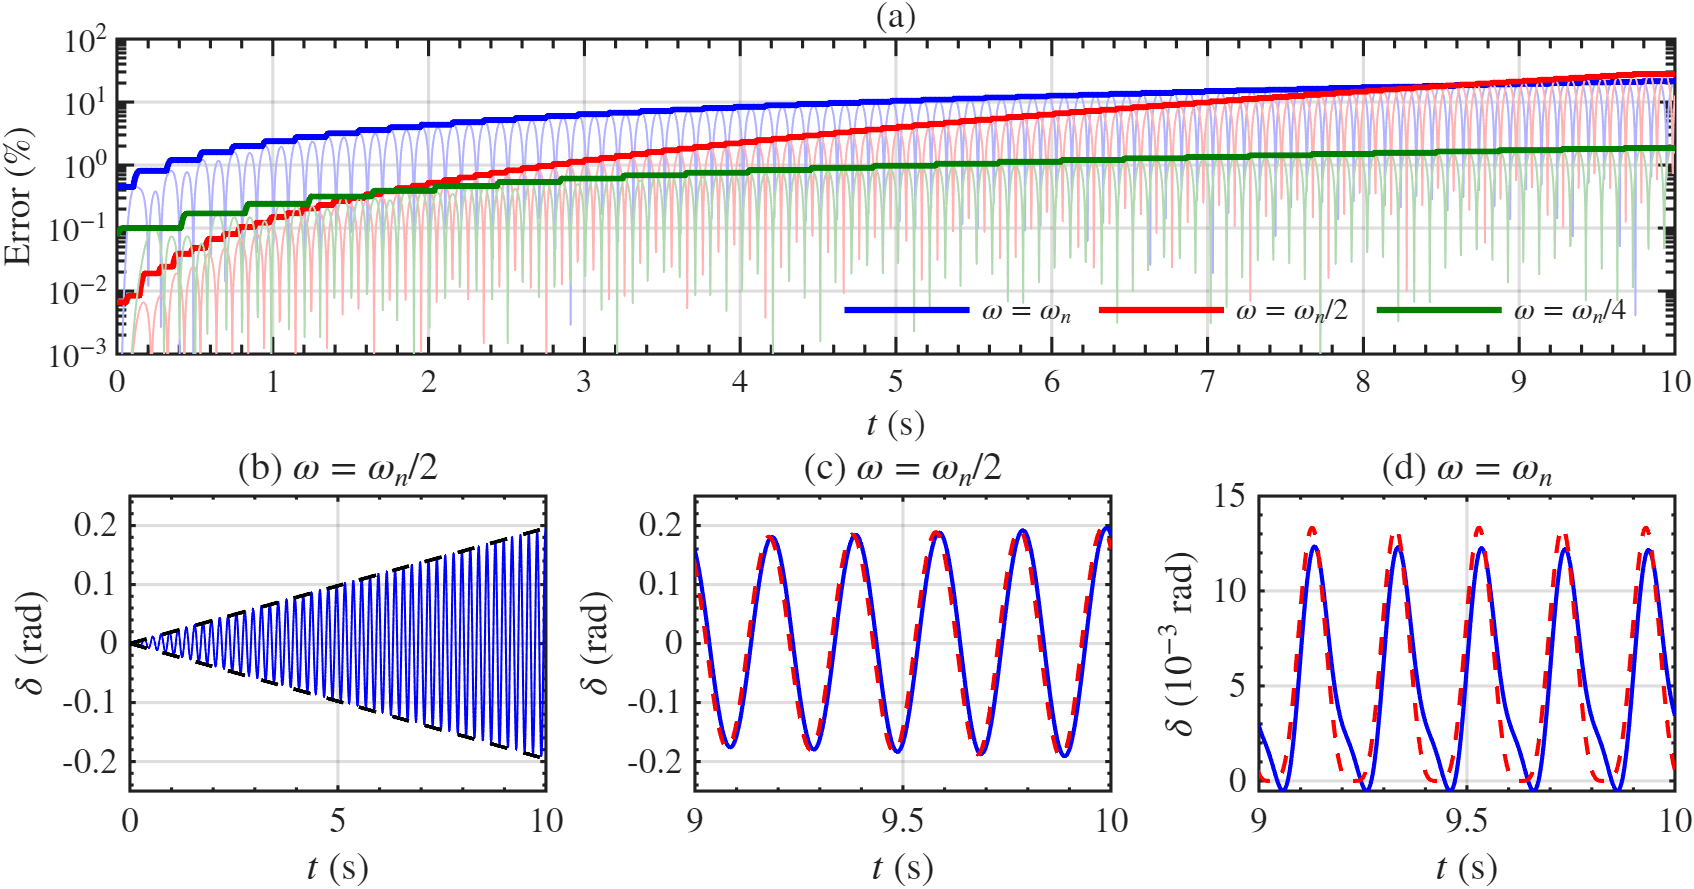
\includegraphics[width=\textwidth]{linearized_error.png}
\caption{(a) Percentage error of the linearized solution (thin: error; thick: its envelope). (b) Full solution at resonance and envelope $\pm F_0t/(2\omega_n)$ (dashed). (c, d) Full solution (solid) and linearized solution (dashed) in the last second.}\label{fig:lin}
\end{figure}

\begin{table}[!htb]
\centering\small
\caption{Linearized against full equation for $\delta(0)=\dot\delta(0)=0$, with $\omega_n=\SI{31.32}{rad/s}$. All errors in \%.}\label{tab:lin}
\begin{tabular}{ccccccc}
\toprule
$\omega$ & $\delta_s$ (rad) & $\max|\delta_{full}|$ (rad) & \multicolumn{2}{c}{Largest error} & \multicolumn{2}{c}{Largest error in $[0,10]$ s, keeping}\\
\cmidrule(lr){4-5}\cmidrule(lr){6-7}
 & & & $[0,5]$ s & $[0,10]$ s & $\Omega^2\delta$ & $\sin\delta$\\
\midrule
$\omega_n$ & 0.00500 & 0.01339 & 10.09 & 21.36 & 0.072 & 21.212\\
$\omega_n/2$ & 0.00125 & 0.19559 & 3.47 & 27.75 & 18.182 & 9.616\\
$\omega_n/4$ & 0.00031 & 0.00083 & 0.90 & 1.86 & 0.001 & 1.860\\
\bottomrule
\end{tabular}
\end{table}

At $\omega=\omega_n/2$ the forcing frequency $2\omega$ equals $\omega_n$: every push of the centrifugal force is in phase with the natural swing, which is the resonance of Eq.~\eqref{eq:res}. The amplitude grows along the line $F_0t/(2\omega_n)$, which gives \SI{0.1958}{rad} at \SI{10}{s} against the \SI{0.19559}{rad} of the full equation (Fig.~\ref{fig:lin}b). So $\delta$ reaches \ang{11.2}, 14.6 times the value at $\omega_n$, although the forcing is 4 times weaker. In Fig.~\ref{fig:lin}a its error starts as the smallest, partly because it is divided by this large final amplitude, and it ends as the largest because as $\delta$ grows the pendulum softens and falls out of phase with the forcing (Fig.~\ref{fig:lin}c). Both approximations contribute: restoring $\sin\delta$ reduces the error from 27.75\% to 9.616\%, and restoring $\Omega^2\delta$ only to 18.182\%. The softening also limits the resonance: integrating the full equation up to \SI{100}{s}, $\delta$ peaks at \SI{0.324}{rad} at $t=\SI{20.5}{s}$, while the linearized envelope reaches \SI{1.96}{rad}.

At $\omega=\omega_n$, $\delta$ stays small and $\sin\delta\approx\delta$ is excellent, but the error still reaches 21.36\%. All of it comes from $\Omega^2\delta$: restoring this term leaves 0.072\%. The term looks negligible, since the mean of $\Omega^2$ is $A^2\omega^2/2=\SI{4.905}{s^{-2}}$, 0.500\% of $g/R$. However, it is a stiffness that varies in time at $2\omega=2\omega_n$, twice the natural frequency (a parametric excitation, which goes beyond the course), and its effect on the natural oscillation builds up swing after swing. A fit of the last second shows the natural part of $\delta_{full}$ \SI{0.41}{rad} behind that of $\delta_{lin}$ and with 0.875 of its amplitude (Fig.~\ref{fig:lin}d), which alone gives an error of 20.0\%. That is why the error doubles from \SI{5}{s} to \SI{10}{s}. At $\omega=\omega_n/4$ the forcing is 16 times weaker than at $\omega_n$ and the error stays below 2\%, so here the linearization can be used. The three cases satisfy $A^2=0.01\ll g/(R\omega^2)=1,4,16$, yet the error differs by more than one order of magnitude: the hypothesis guarantees that the neglected term is small in the equation, not that its effect stays small in time.

\subsection{Limits of the Model}
The wire has no friction and nothing removes energy. Even so, only the linearized equation grows without limit: the full one is limited by its softening, and real damping would reduce the amplitude further \cite[Sec.~5.4.1]{notes}. The rotation of the plane is imposed, which assumes a motor able to give the torque $|xN_2|$ (up to \SI{3.422}{N.m} here) whatever $P$ does. The wire is bilateral: $N_1$ and $N_2$ can take either sign, so unlike the string of Lab 1 no event ends the motion. Finally, Table~\ref{tab:lin} holds for our choice of initial conditions: with $\delta(0)=\SI{0.1}{rad}$ the largest errors rise to 55\%, 43\% and 24\%, because the free oscillation is larger, so the conclusion at $\omega_n/4$ is only valid for $P$ starting at rest at the bottom.

\section{Conclusions}\label{sec:conc}
\begin{itemize}[noitemsep,topsep=2pt]
\item The particle has one degree of freedom, and Eq.~\eqref{eq:eom} contains only gravity and the centrifugal force. The Coriolis force is the largest inertia force, but it only loads the wire, through $N_2$. For $\omega=\SI{0.1}{rad/s}$ the rotation is slow, and $P$ swings as a pendulum of \ang{90} amplitude with the wire carrying up to $3mg$ in its plane.
\item The mechanical energy is not conserved because the moving wire does work. The motor gives and takes back the energy needed to change the angular momentum about the axis, so $E$ oscillates with each swing but has almost no net gain after each period of the plane.
\item On a fixed loop, energy gives the critical rate $\dph_c=\sqrt{(2g/R)(1-\sin\varphi_0)}$, which all the simulated cases confirm. Only three of the nine initial conditions rotate.
\item The linearized equation is a forced oscillator with a resonance at $\omega=\tfrac12\sqrt{g/R}$, where $\delta\ll1$ fails. It also loses accuracy away from resonance, since a term that is small in the equation builds up in time. Only the weakest forcing, starting at rest at the bottom, keeps the error below 2\%.
\end{itemize}

{\footnotesize
\bibliographystyle{unsrt}
\bibliography{references}}
\end{document}
